\documentclass{beamer}

\usepackage{amssymb,amsthm,amsmath} %ams
\usepackage[finnish]{babel} %suomenkielinen tavutus
\usepackage[T1]{fontenc} %skanditavutus
\usepackage[utf8x]{inputenc}        	% skandit utf-8 koodauksella
\usepackage{graphicx}
\usepackage{tikz}% vähän tehokkaampi grafiikkapaketti
\usepackage[square]{natbib}
\usepackage{subcaption} % for side by side figures

\begin{document}

\frame{
 \frametitle{Avaruusjakoon perustuvat tietorakenteet tietokonegrafiikassa}
 \framesubtitle{LuK-tutkielma, Timo Heinonen, 20. joulukuuta 2016}
 \begin{itemize}
  \item{Kirjallisuuskatsaus}
  \item{Työn päämäärä:}
  \begin{itemize}
   \item{Esitellä säteenseurannan rooli tietokonegrafiikassa}
   \item{Esitellä tietorakenteita, joiden avulla säteenseurantaa voidaan nopeuttaa}
   \item{Vertailla tietorakenteita keskenään}
  \end{itemize}
 \end{itemize}
}

\frame{
  \frametitle{Tärkeimmät lähteet}
  \begin{itemize}
    \item{Klassikot}
    \begin{itemize}
      \item{Appel, A. (1968). \emph{Some techniques for shading machine renderings of solids}}
      \item{Fuchs, H., Kedem, Z. M., ja Naylor, B. F. (1980). \emph{On visible surface generation by a priori tree structures}}
    \end{itemize}
    \item{Oppikirjat}
    \begin{itemize}
      \item{Janke, S. J. (2015). \emph{Mathematical Structures for Computer Graphics}}
      \item{Hughes, J. F. et al. (2013). \emph{Computer graphics: principles and practice}}     
%\item{Harju, T. (1989-2015). \emph{Geometria, lyhyt kurssi, Turun yliopisto}}
      \item{Samet, H. (2005). \emph{Foundations of Multidimensional and Metric Data Structures}}
    \end{itemize}
    \item{Tutkimusta tietorakenteiden vertailusta}
    \begin{itemize}
      \item{Havran, V. (2000). \emph{Heuristic Ray Shooting Algorithms, väitöskirja}}
      \item{Wald, I. (2004). \emph{Realtime Ray Tracing and Interactive Global Illumination, väitöskirja}}
      \item{Thrane, N. ja Simonsen, L. O. (2005). \emph{A comparison of acceleration structures for gpu assisted ray tracing, pro gradu -työ}}
    \end{itemize}
  \end{itemize}
}

\frame{
 \frametitle{Käsitteitä}
 \begin{itemize}
  \item{\textbf{\emph{hahmontaminen}} (engl. \emph{rendering}): luo kolmiulotteisesta maisemasta kaksiulotteisen kuvan}

  \item{\textbf{\emph{maisema}} (engl. \emph{scene}): joukko geometrisesti määriteltyjä \emph{objekteja}, esimerkiksi hahmo, rakennus, puu..., ja valonlähteitä}

  \item{\textbf{\emph{monikulmio}} (engl. \emph{polygon}): objektit on usein jaettu pienempiin osiin, useimmiten kolmioihin hahmontamisen helpottamiseksi}

  \item{\textbf{\emph{säteenseuranta}} (engl. \emph{ray tracing}): hahmontamistekniikka, joka mallintaa valonsäteiden kulkua maisemassa. Tuottaa erittäin realistisia kuvia}
 \end{itemize}
}

\frame{
 \frametitle{Käsitteitä}
 \begin{figure}
  \centering 
  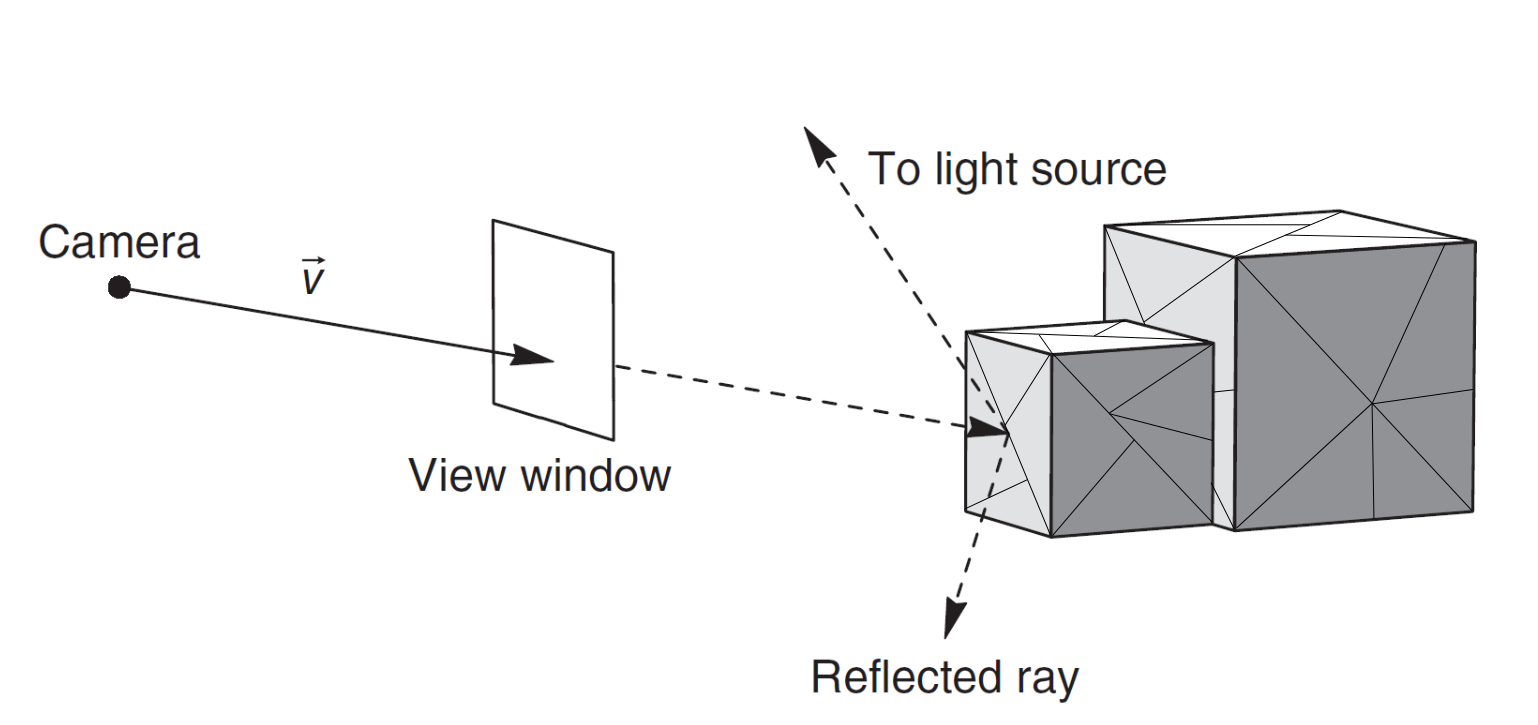
\includegraphics[width=0.8\textwidth]{img/raytracingtri.png}
  \caption{Säteenseuranta \citep{janke}}
  \label{raytracing}
  \vspace{-0.5cm}
 \end{figure}
}

\frame{
 \frametitle{Säteenseuranta on hidasta}
 \begin{itemize}
  \item{Säteenseurannassa jokaista pikseliä kohti on ammuttava säde maisemaan ja testattava sen yhteentörmäystä jokaiseen monikulmioon}
  \item{$O(mn)$ yhteentörmäystestiä, missä $m$ on kuvan pikselien, ja $n$ maiseman monikulmioiden määrä}
  \item{Yhteentörmäysten selvittämiseen voi kulua jopa 95\% koko laskenta-ajasta \citep{whitted}}
  \item{Työtä voidaan siirtää esiprosessointivaiheeseen muodostamalla maisemasta hierarkinen tietorakenne}
%  \item{Tavoitteena on vähentää testien määrää luokkaan $O(m \log n)$}
 \end{itemize}
}

\frame{
 \frametitle{Monsterit yliopisto}
 \begin{figure}
  \centering 
  
\includegraphics[width=\textwidth]{img/monsters.jpg}
  \caption{\url{http://www.nerdist.com/wp-content/uploads/2013/06/monsters1.jpg}}
  \label{monsters}
 \end{figure}
}

\frame{
 \frametitle{BSP-puu}
 \begin{figure}%[htp]
  \centering
  \begin{subfigure}{0.5\textwidth} 
% \centering
   \def\svgwidth{0.95\linewidth}
   \input{img/bsp11.pdf_tex}
   \caption{Joukko monikulmioita tasossa}
   \label{bsp11}
  \end{subfigure}%
 \begin{subfigure}{0.5\textwidth} 
 % \centering
  \def\svgwidth{0.95\linewidth}
  \input{img/bsp12.pdf_tex}
  \caption{Taso neljän jaon jälkeen}
  \label{bsp12}
 \end{subfigure}
 \caption{Tason jakaminen}
 \vspace{-0.5cm}
 \label{bsp1}
\end{figure}
}

\frame{
 \frametitle{BSP-puu}
 \begin{figure}
  \centering
  \begin{figure}
 \centering
 \begin{tikzpicture}[level/.style={sibling distance = 60mm/#1}]
  \node[circle,draw] (z){$G$}
    child {node [circle,draw] (a) {$E$}
     child {node [circle,draw] (b) {$D$}}
     child {node [circle,draw] (c) {$F$}}
    }
    child {node [circle,draw] (d) {$B$}
     child {node [circle,draw] (e) {$C_2$}}
     child {node [circle,draw] (f) {$A$}
      child[missing] {node {}}
      child {node [circle,draw] (g) {$C_1$}}}
    };
 \end{tikzpicture}
 \caption{Tasosta muodostettu BSP-puu}
 %\vspace{-0.5cm}
 \label{bsp2}
\end{figure}

%  \label{bsp2}
 \end{figure}
}

\frame{
 \frametitle{kd-puu}
 \begin{figure}
  \centering 
  \def\svgwidth{0.8\linewidth}
  \input{img/kd1.pdf_tex}
  \caption{Taso jaettuna kuusi kertaa koordinaattiakselien suuntaisesti}
  \vspace{-0.5cm} 
  \label{bsp3}
 \end{figure}
}

\frame{
 \frametitle{kd-puu}
 \begin{figure}
  \centering
  \begin{figure}
 \centering
 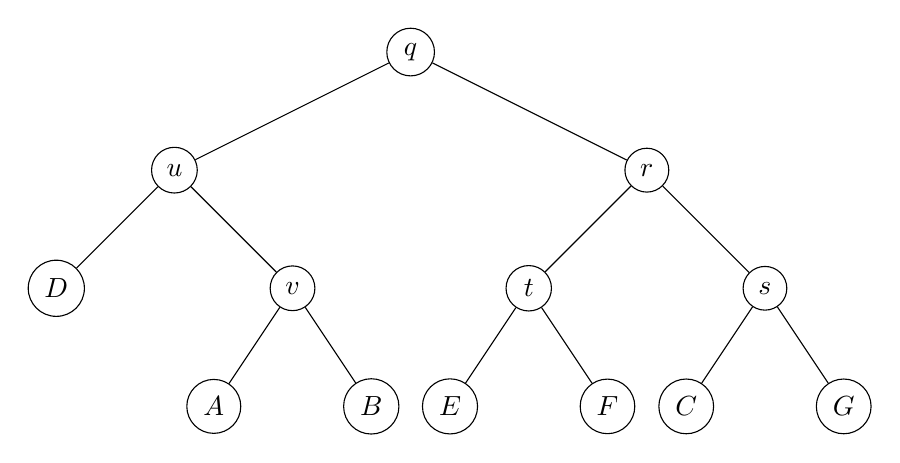
\begin{tikzpicture}[level/.style={sibling distance = 60mm/#1}]
  \node[circle,draw] (z){$q$}
   child {node [circle,draw] (a) {$u$}
    child {node [circle,draw] (b) {$D$}}
    child {node [circle,draw] (c) {$v$}
     child {node [circle,draw] (d) {$A$}}
     child {node [circle,draw] (e) {$B$}}
    }
   }
   child {node [circle,draw] (f) {$r$}
    child {node [circle,draw] (g) {$t$}
     child {node [circle,draw] (h) {$E$}}
     child {node [circle,draw] (i) {$F$}}
    }
    child {node [circle,draw] (j) {$s$}
     child {node [circle,draw] (k) {$C$}}
     child {node [circle,draw] (l) {$G$}}
    }
  };
 \end{tikzpicture}
 \caption{Tasosta muodostettu kd-puu}
 \label{bsp4}
\end{figure}

%  \label{bsp4}
  \end{figure}
}

\frame{
 \frametitle{Rajaavat tilat}
 \begin{figure}[htp]
  \centering 
  \def\svgwidth{0.8\linewidth}
  \input{img/bvhfancy.pdf_tex}
  \caption{Objektijoukko jaettuna rajaaviin tiloihin}
  \vspace{-0.5cm} 
  \label{bvh}
 \end{figure}
}

\frame{
 \frametitle{BVH, Bounding Volume Hierarchy}
 \begin{figure}
  \centering
   \begin{figure}[htp]
 \centering
 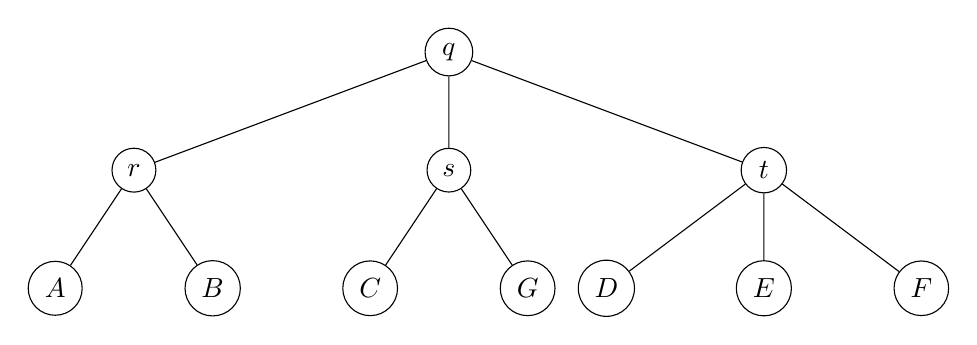
\begin{tikzpicture}[level/.style={sibling distance = 40mm/#1}]
  \node[circle,draw] (z){$q$}
    child {node [circle,draw] (a) {$r$}
     child {node [circle,draw] (b) {$A$}}
     child {node [circle,draw] (c) {$B$}}
    }
    child {node [circle,draw] (d) {$s$}
     child {node [circle,draw] (e) {$C$}}
     child {node [circle,draw] (f) {$G$}}
    }
    child {node [circle,draw] (g) {$t$}
     child {node [circle,draw] (h) {$D$}}
     child {node [circle,draw] (i) {$E$}}
     child {node [circle,draw] (j) {$F$}}
    };
 \end{tikzpicture}
 \caption{Objektijoukosta muodostettu BVH-puu}
 \vspace{-0.5cm}
 \label{bvhtree}
\end{figure}

 % \label{bvhtree}
 \end{figure}
}

\frame{
 \frametitle{Tietorakenteiden vertailua}
 \begin{itemize}
  \item{Tietorakenteet on alustettava huolellisesti, jotta niistä olisi mahdollisimman paljon hyötyä}
  \item{Ongelmia:}
  \begin{itemize}
   \item{BSP- ja kd-puissa monikulmioiden määrän lisääntyminen}
   \item{BVH:ssa liian löyhät rajaavat tilat}
  \end{itemize}
  \item{Tietorakenteiden käyttö säteenseurannassa on hyvin samankaltaista}
  \begin{itemize}
   \item{Mikäli maisemaan ammuttu säde osuu tietorakenteen solmun määrittämään avaruuden osaan, jatketaan tarkastelua solmun lapsiin}
  \end{itemize}
 \end{itemize}
}

\frame{
  \frametitle{Tietorakenteiden vertailua}
  \begin{itemize}
   \item{Eräässä vertailussa kd-puu toi suurimman nopeutuksen hahmontamiseen ja BVH pienimmän \citep{havran}}
   \item{Toisaalta toisessa vertailussa BVH:n avulla saavutettiin yhdeksänkertainen nopeutus kd-puuhun verrattuna \citep{thrane}}
   \item{Parasta tietorakennetta ei pystytä osoittamaan, sillä käytännössä tietorakenteen tuoma hyöty riippuu maisemasta, laitteistosta, implementaatiosta ja sovelluksesta}
   \item{\underline{Keskimäärin yhteentörmäystestien määrä: $O(n) \rightarrow O(\log n)$}}
  \end{itemize}
}

%\frame{
% \frametitle{Tietorakenteiden alustamisen vertailua}
% \begin{itemize}
%  %\item{\cite{wald01}}
%  \item{Muodostettaessa BSP- ja kd-puita voidaan joutua jakamaan monikulmioita osiin tai sisällyttämään ne useaan solmuun. Tämä kasvattaa puun kokoa ja siten hidastaa sen läpikäyntiä}
%  \item{BVH:ta alustettaessa samaa ongelmaa ei synny}
%  \item{Ingo Waldin tutkimuksessa BVH:n muodostaminen oli jopa 10 kertaa nopeampaa kuin kd-puun \citep{wald07}}
% \end{itemize}
%}

%\frame{
% \frametitle{Tietorakenteiden käytön vertailua}
% \begin{itemize}
%  \item{Tietorakenteiden käyttäminen hahmontamisessa on hyvin samankaltaista: jos säde ei osu solmun määrittämään avaruuden osaan, voidaan tarkastelu lopettaa}
%  \item{Eräässä vertailussa kd-puu toi suurimman nopeutuksen hahmontamiseen ja BVH pienimmän \citep{havran}}
%  \item{Toisaalta toisessa vertailussa BVH:n avulla saavutettiin yhdeksänkertainen nopeutus kd-puuhun verrattuna \citep{thrane}}
%  \item{Käytännössä tietorakenteen tuoma hyöty riippuu maisemasta, laitteistosta, implementaatiosta ja sovelluksesta}
%  \item{\underline{Keskimäärin yhteentörmäystestien määrä: $O(n) \rightarrow O(\log n)$}}
% \end{itemize}
%}

%\frame{
% \frametitle{Reaaliaikainen säteenseuranta}
% \begin{itemize}
%  \item{Jotta säteenseurantaa voitaisiin käyttää reaaliaikaisesti esimerkiksi videopeleissä ja virtuaalitodellisuudessa, tulisi hahmontaa ja näyttää yli 30 kuvaa sekunnissa}
%  \item{Staattisille maisemille tämä on mahdollista}
%  \item{Maisemat, jossa objektit liikkuvat ovat ongelmallisempia: avaruuden jakavaa tietorakennetta joudutaan päivittämään}
%  \item{Uusi kd-puu voidaan rakentaa maisemasta ajassa $O(n \log n)$, mutta tämä ei ole tarpeeksi nopeaa}
%  \item{Parempi tapa näyttäisi olevan BVH:n rajaavien tilojen koordinaattien päivittäminen kuvien välissä}
% \end{itemize}
%}

\bibliographystyle{apalike-finnish} %apalike-finnish

\frame{
 \frametitle{Viitteet}
 \bibliography{bibliography}
}

\end{document}
